\documentclass[12pt,a4paper]{article}
\usepackage[margin=2.5cm]{geometry}
\usepackage[utf8]{inputenc}
%\usepackage[ngerman]{babel}
\usepackage{amscd}
\usepackage{amsmath}
\usepackage{amssymb}
\usepackage{amsfonts}
\usepackage{amsthm}
%\usepackage{ntheorem}
\usepackage{graphicx}
\usepackage{picinpar}
\usepackage{enumerate}
\usepackage{hyphenat}
\usepackage{mathrsfs}
\usepackage{cancel}
\usepackage{enumitem}
\usepackage{bbm}
\usepackage{fancyhdr}
\usepackage{comment}
\usepackage{nameref}
\usepackage{float}
\usepackage{listings}
\usepackage{appendix}
\usepackage{hyperref}

\pagestyle{fancy}






% bei jeder section neue seite beginnen
\let\stdsection\section
\renewcommand\section{\cleardoublepage\stdsection}

\newcommand{\superscript}[1]{\ensuremath{^{\textrm{#1}}}}
\newcommand{\subscript}[1]{\ensuremath{_{\textrm{#1}}}}

\newcommand{\unit}[1]{\ensuremath{\,\mathrm{#1}}}
\newcommand{\myPath}[1]{{\small\texttt{#1}}}
\newcommand{\function}[1]{{\small\texttt{#1}}}
\newcommand{\commandline}[1]{{\small\texttt{#1}}}
\newcommand{\keyword}[1]{{\small\texttt{#1}}}

\renewcommand{\arraystretch}{1.5}


\usepackage{color}
 
\definecolor{dkgreen}{rgb}{0,0.6,0}
\definecolor{gray}{rgb}{0.5,0.5,0.5}
\definecolor{mauve}{rgb}{0.58,0,0.82}
\lstset{
	language=Python,
	numbers=left,
	showstringspaces=false,
	frame=single,
	captionpos=b,
	breaklines=true,
	breakatwhitespace=false,
	title=\lstname,
	keywordstyle=\color{blue},          % keyword style
	commentstyle=\color{dkgreen},       % comment style
	stringstyle=\color{mauve}, 
}



\begin{document}
\title{TXL Wizard: Reference Manual}
\author{Esteban Marín}
\date{2016-05-13}
\maketitle


\newpage
\tableofcontents
\pagestyle{headings}

\newpage



\section{Introduction}
    This document describes the usage and technical reference of the python program ``TXLWizard''
    written by Esteban Marin (\href{mailto:estebanmarin@gmx.ch}{estebanmarin@gmx.ch}).\\

    \subsection{What does it do?}
        The ``TXLWizard'' provides routines for generating TXL files (.txl) for
        the preparation of E-Beam lithography masks using python code. The TXL files can be processed with BEAMER.
        See the following links:
        \begin{itemize}
            \item \url{http://genisys-gmbh.com/web/products/beamer.html}
            \item \url{http://cad035.psi.ch/LB_index.html}
            \item \url{http://cad035.psi.ch/LBDoc/BEAMER_Manual.pdf}
        \end{itemize}
        The generated TXL files are also converted to HTML / SVG for presentation in any modern browser or
        vector graphics application.\\
        Moreover, a command line interface ``TXLConverter'' provides conversion of existing TXL files to HTML / SVG
        (See Section \ref{sec:TXLConverter}).


    \subsection{Technical Information}
        The ``TXLWizard'' is written in python and will run in Python version 2.7+ and 3.1+.\\
        In order to use the ``TXLWizard'', package must be available as
        a python package, i.e. either it must be copied to \myPath{Path\_to\_my\_python\_installation/site-packages/} or
        to the path where your script is located. \\
        Alternatively, you can also prepend the following command to your python script:\\
        \commandline{sys.path.append('path to the folder containing TXLWizard')}\\





\section{TXLWizard Example}
The following code demonstrates a simple example usage of the ``TXLWizard''.
The resulting image is shown in Figure \ref{fig:TXLWizardSimpleExample}.
A more advanced example is shown in Section \ref{sec:AppendixTXLWizardExampleAdvanced}
\lstinputlisting[language=Python]{Content/Example_Simple.py}


\begin{figure}[!htbp]
    \centering
     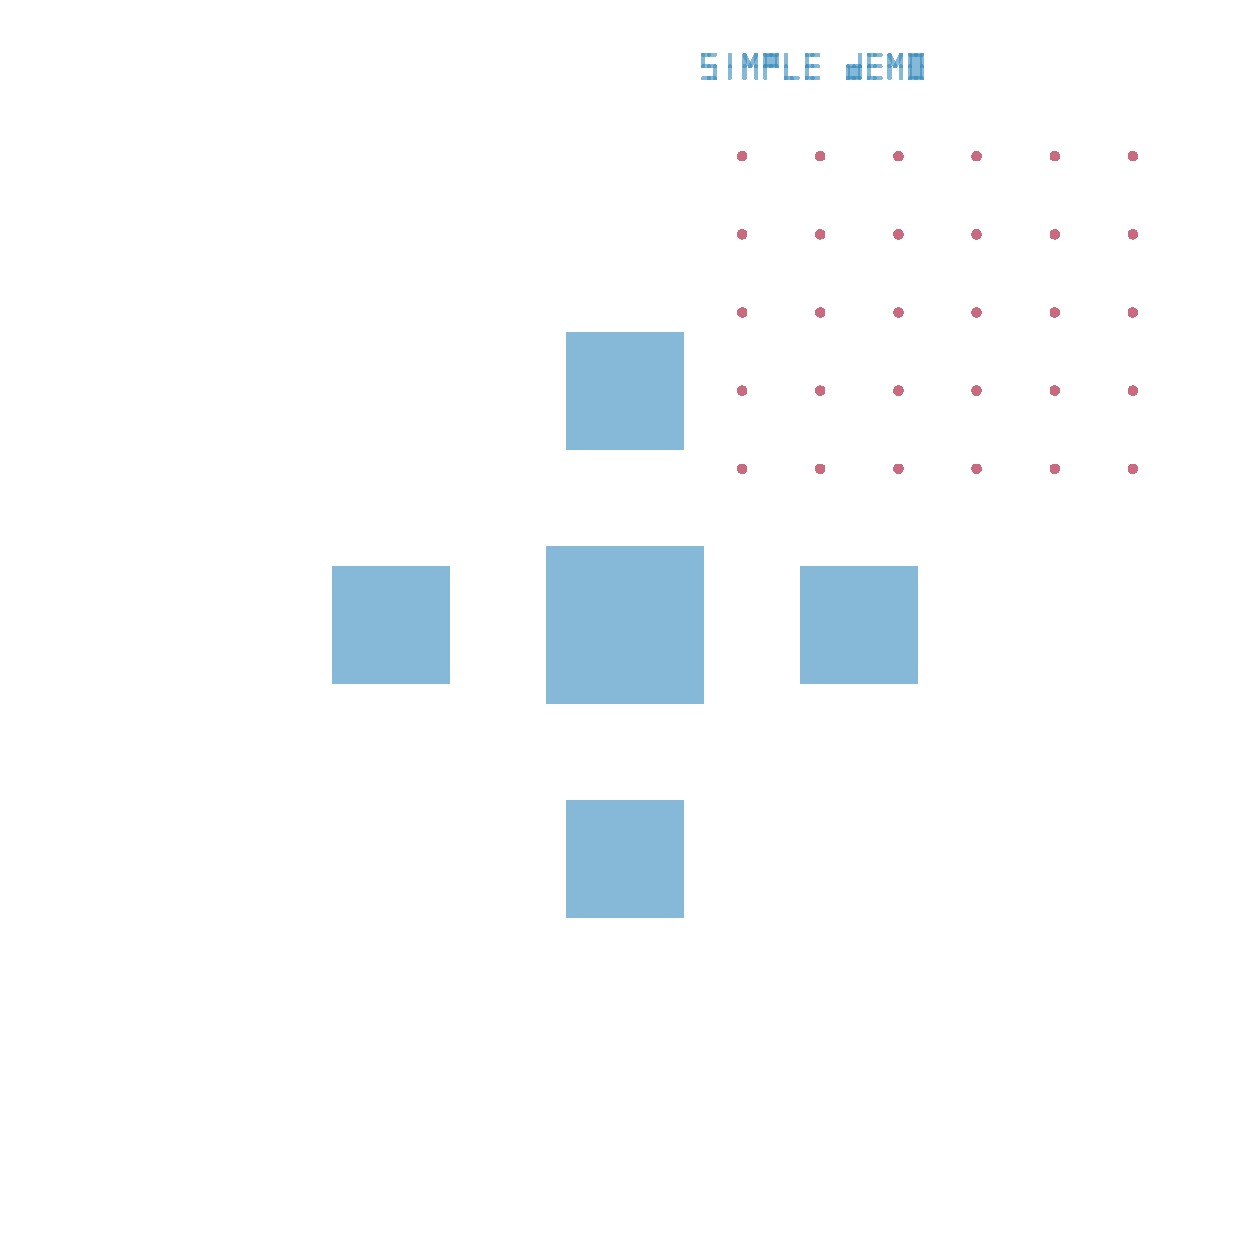
\includegraphics[width=\textwidth]{Content/Masks/EM160509_Demo_Simple.pdf}
    \caption{Simple Example: Generated Mask}
    \label{fig:TXLWizardSimpleExample}
\end{figure}
\section{Class Reference}
    \subsection{TXLWizard.TXLWriter}
        \subsubsection{Description}
            Controller class for generating TXL / SVG / HTML output.
            Here we can add structures (definitions and content) which will be rendered in the output.
        \subsubsection{Methods}
            \paragraph{\_\_init\_\_}
                \subparagraph{Description} Constructor method
                \subparagraph{Parameters}\mbox \\
                    \textit{Keyword Arguments}
                    \begin{itemize}
                        \item \textbf{Width}\superscript{*} \keyword{int} Width of the sample in um. Used to draw coordinate system.
                        \item \textbf{Height}\superscript{*} \keyword{int} Height of the sample in um. Used to draw coordinate system.
                        \item \textbf{ShowCoordinateSystem}\superscript{*} \keyword{bool} Show the coordinate system or not
                        \item \textbf{GridDistance}\superscript{*} \keyword{int} Coordinate Sytem Grid Spacing in um.
                        \item \textbf{SubGridDistance}\superscript{*} \keyword{int} Coordinate System Sub-Grid Spacing in um
                    \end{itemize}
        \subsubsection{Properties}
        \subsubsection{Example Usage}
            \begin{lstlisting}
import TXLWizard.TXLWriter

TXLWriter = TXLWizard.TXLWriter.TXLWriter(
    Width=500,
    Height=400
)
            \end{lstlisting}

    \subsection{Strukturen}
        \subsubsection{DataStructure}
            Die DataStructure ist wie folgt definiert und gilt jeweils für eine Datenbank-Tabelle:
            \begin{itemize}
                \item \textbf{Control}
                    \keyword{Array} mit Informationen zur Datentabellen-Kontrolle.
                    \begin{itemize}
                        \item \textbf{Table}\superscript{*} \keyword{String} Tabellen-Name
                        \item \textbf{IndexColumn}\superscript{*} \keyword{String} Name der Index-Spalte. Standardwert: ``ID''
                        \item \textbf{ModifiedTSColumn}\superscript{*} \keyword{String} Name der Spalte mit Änderungs-Timestamp. Standardwert: ``ModifiedTS''
                        \item \textbf{CategoryColumn}\superscript{*} \keyword{String} Name der Kategorien-Spalte. Falls angegeben (muss vom \textbf{Type} \textbf{Module} mit \textbf{DataCardinality} ``1:n'' sein), kann nach
                        dieser Spalte kategorisiert werden. (z.B. select-Feld, etc.) Standardwert: ``ID''
                        \item \textbf{NoUserInput}\superscript{*} \keyword{Bool} Ob kein User-Input in die Daten gelangen darf. Standardwert:  \keyword{false}
                        \item \textbf{ReadOnly}\superscript{*} \keyword{Bool} Ob Datenbank-Tabelle schreibgeschützt ist. Standardwert:  \keyword{false}
                        \item \textbf{NoPurge}\superscript{*} \keyword{Bool} Ob gelöschte Einträge in Datenbank-Tabelle nicht gelöscht werden sollen. Standardwert:  \keyword{false}
                        \item \textbf{DBConnectionID}\superscript{*} \keyword{String} Name der Datenbankverbindung. Standardwert: ``ClusterNetAppDB''

                    \end{itemize}
                \item \textbf{Columns}
                    \keyword{Array} mit Definitionen der einzelnen Daten-Spalten.
                    \keyword{Key} ist der Spalten-Name und \keyword{Value} ein \keyword{Array} mit der Definition:
                    \begin{itemize}
                        \item \textbf{Type} \keyword{String} Typ der Spalte. Kann folgende Werte annehmen:
                            \begin{itemize}
                                \item \textbf{Integer} Ganzzahl
                                \item \textbf{String} Text
                                \item \textbf{Float} Gleitkommazahl
                                \item \textbf{Checkbox} Checkbox
                                \item \textbf{Date} Datum
                                \item \textbf{Time} Zeit
                                \item \textbf{DateTime} Datum und Uhrzeit
                                \item \textbf{Array} \keyword{Array}, wird als JSON gespeichert.
                                \item \textbf{Module} Fremdschlüssel (ID, Referenz) zu einem Eintrag in einem anderen Modul.
                                \item \textbf{FileResource} Dateien
                                \item \textbf{Option} Mehrfachauswahl

                            \end{itemize}
                            Wird \textbf{Type} nicht angegeben, so wird in \commandline{\$GLOBALS['DefaultFieldStructures']} nach einem Eintrag gesucht. In diesem Fall kann lediglich der \textbf{DefaultValue} erhalten bleiben.
                        \item \textbf{Validation}\superscript{*} \keyword{Array} mit Validierungs-Optionen.
                            \begin{itemize}
                                \item \textbf{Required}\superscript{*} \keyword{Bool} Ob Pflichtfeld. Standardwert: \keyword{false}
                            \end{itemize}
                        \item \textbf{LabelKey}\superscript{*} \keyword{String} Key für Language Label. Standardwert: ``''
                        \item \textbf{TypeSpecificConfiguration}\superscript{*} \keyword{Array} spezifische Konfiguration (abhängig von \textbf{Type}) \\
                            \-\hspace{2mm}\textit{\textbf{Type} ``Module''}
                            \begin{itemize}
                                \item \textbf{ModulePath} \keyword{String} Pfad des Moduls
                                \item \textbf{MModulePath}\superscript{*}  \keyword{String} Pfad des M-Moduls der n:m-Relation (benötigt für \textbf{DataCardinality} ``n:m'')
                                \item \textbf{DataCardinality}\superscript{*} \keyword{String} Kardinalität. Erlaubt: ``1:n'', ``n:m'', Standardwert: ``1:n''
                                \item \textbf{NToMTable}\superscript{*} \keyword{String} Tabelle für n:m-Relation. (benötigt für \textbf{DataCardinality} ``n:m'')
                                \item \textbf{NForeignKeyColumn}\superscript{*} \keyword{String} Foreign Key Spalte n:m-Relation (n-Tabelle). (benötigt für \textbf{DataCardinality} ``n:m'')
                                \item \textbf{MForeignKeyColumn}\superscript{*} \keyword{String} Foreign Key Spalte für n:m-Relation. (m-Tabelle) (benötigt für \textbf{DataCardinality} ``n:m'')
                                \item \textbf{ModuleInstance}\superscript{*} \keyword{Reference} Referenz zu einer Modul-Instanz. Falls leer, wird diese anhand des \textbf{ModulePath} erzeugt.
                                \item \textbf{MModuleInstance}\superscript{*} \keyword{Reference} Referenz zu einer M-Modul-Instanz. Falls leer, wird diese anhand des \textbf{ModulePath} erzeugt. (für \textbf{DataCardinality} ``n:m'')
                                \item \textbf{ReplicateToJS}\superscript{*} \keyword{Bool} ob Javascript-Modul-Instanz erstellt werden soll. Standardwert: \keyword{false}
                                \item \textbf{OverrideInstanceProperties}\superscript{*} \keyword{Array} Eigenschaften, die bei Instanziierung des Objekts gesetzt werden sollen. Standardwert: leeres \keyword{Array}
                                \item \textbf{OverrideForeignInstanceProperties}\superscript{*} \keyword{Array} Eigenschaften, die bei Instanziierung des M-Objekts gesetzt werden sollen. (für \textbf{DataCardinality} ``n:m'') Standardwert: leeres \keyword{Array}
                                \item \textbf{DetailViewType}\superscript{*} \keyword{String} Anzeigemodus in der Detailansicht. (für \textbf{DataCardinality} ``n:m''). Erlaubte Werte: ``Full'', ``Minimal'' Standardwert: ``Minimal''
                                \item \textbf{OptionListAdditionalColumns}\superscript{*} \keyword{Array} Spalten, die beim Select-option zusätzlich im Frontend vorhanden sein sollen (für \textbf{DataCardinality} ``1:n''). Standardwert: leeres \keyword{Array}
                                \item \textbf{RequirePermission} \keyword{Bool} ob relationaler Eintrag gelesen werden können muss, um Datensatz zu lesen. Standardwert: \keyword{false}
                            \end{itemize}

                            \-\hspace{2mm}\textit{\textbf{Type} ``Date''}
                            \begin{itemize}
                                \item \textbf{AddCurrentTimeToInputDate}\superscript{*} \keyword{Bool} ob beim Parsen von User-Input die aktuelle Uhrzeit mitgespeichert werden soll. Standardwert: \keyword{false}
                            \end{itemize}

                            \-\hspace{2mm}\textit{\textbf{Type} ``String''}
                            \begin{itemize}
                                \item \textbf{EncryptDBContent}\superscript{*} \keyword{Bool} Ob Wert in der Datenbank verschlüsselt werden soll. Standardwert: \keyword{false}
                                \item \textbf{RichText}\superscript{*} \keyword{Bool} Ob Rich Text editing \& anzeige aktiviert ist. Standardwert: \keyword{false}
                                \item \textbf{AdditionalAllowedHTMLTags}\superscript{*} \keyword{String} Weitere erlaubte Tags. Standardwert: ``''
                            \end{itemize}

                            \-\hspace{2mm}\textit{\textbf{Type} ``FileResource''}
                            \begin{itemize}
                                \item \textbf{IsCollection}\superscript{*} \keyword{Bool} Ob mehrere Dateien. Standardwert: \keyword{false}
                            \end{itemize}

                            \-\hspace{2mm}\textit{\textbf{Type} ``Integer''}
                            \begin{itemize}
                                \item \textbf{RoundingFactor}\superscript{*} \keyword{Float} Rundungsfaktor. Standardwert: $1$
                            \end{itemize}

                            \-\hspace{2mm}\textit{\textbf{Type} ``Float''}
                            \begin{itemize}
                                \item \textbf{RoundingFactor}\superscript{*} \keyword{Float} Rundungsfaktor. Standardwert: $1$
                            \end{itemize}

                            \-\hspace{2mm}\textit{\textbf{Type} ``Checkbox''}
                            \begin{itemize}
                                \item \textbf{YesNoLabelKeys}\superscript{*} \keyword{Array} spezielle Yes/No Label Keys. Standardwert: leeres \keyword{Array}
                            \end{itemize}

                             \-\hspace{2mm}\textit{\textbf{Type} ``Option''}
                             \begin{itemize}
                                 \item \textbf{Options} \keyword{Array} Optionen, jede es Element ein \keyword{Array} (ID => 'ID', LabelKey => 'LabelKey')
                             \end{itemize}
                        \item \textbf{Visible}\superscript{*} \keyword{Bool} sichtbar? Standardwert: \keyword{true}
                        \item \textbf{DefaultValue}\superscript{*} \keyword{String} Initialwert. Standardwert: \textbf{Type}-abhängigen Standardwert gesetzt.
                        \item \textbf{Update}\superscript{*} \keyword{Bool} ob Feld bei Update in DB geschrieben wird. Standardwert: \keyword{true}
                        \item \textbf{Insert}\superscript{*} \keyword{Bool} ob Feld bei Insert in DB geschrieben wird. Standardwert: \keyword{true}
                        \item \textbf{NoUserInput}\superscript{*} \keyword{Bool} Ob Feld keine Benutzer-Eingaben erhalten darf. Standardwert: \keyword{false}
                        \item \textbf{DisplayOptions}\superscript{*}
                            Anzeigeoptionen. Wird an Form übergeben. Standardwert: leeres \keyword{Array}
                            \begin{itemize}
                                \item \textbf{IsPassword}\superscript{*} \keyword{Bool} ob Textfeld als Password dargestellt werden soll. Standardwert: \keyword{false}
                                \item \textbf{IsCurrency}\superscript{*} \keyword{Bool} ob Textfeld als Währung dargestellt werden soll. Bsp: \verb+2'700.35+ Standardwert: \keyword{false}
                                \item \textbf{IsLanguageLabelKey}\superscript{*} \keyword{Bool} ob es ein Language Label Key ist. (für \textbf{type} \textbf{String}) Standardwert: \keyword{false}
                                \item \textbf{Multiline}\superscript{*} \keyword{Bool} ob mehrzeiliges Textfeld (nur für \textbf{String}) Standardwert: \keyword{false}
                                \item \textbf{FormRowCSSClasses}\superscript{*} \keyword{String} zusätzliche Klassen für Formular-Zeile. Standardwert: ``''
                                \item \textbf{CSSClasses}\superscript{*} \keyword{String} zusätzliche Klassen für Formular-Feld. Standardwert: ``''
                                \item \textbf{LinkURLs}\superscript{*} \keyword{Bool} ob URLs im Inhalt gesucht und verlinkt werden sollen (nur für \textbf{String}) Standardwert: \keyword{false}
                                \item \textbf{DateFormat}\superscript{*} \keyword{String} Datumsformat für ``Date''-Feld. Standardwert: ``d.m.Y''
                            \end{itemize}
                        \item \textbf{FormFieldParameters}\superscript{*} \keyword{Array} Parameter, die an das Formular-Objekt übergeben werden. Standardwert: leeres \keyword{Array}
                            \begin{itemize}
                                \item \textbf{IsTabFocusField}\superscript{*} \keyword{Bool} ob Textfeld im aktuellen Tab standardmässig fokussiert sein soll. Standardwert: \keyword{false}
                            \end{itemize}
                        \item \textbf{SessionPersistent}\superscript{*} \keyword{Bool} Ob Wert der Variable Session-persistent gespeichert werden soll. Standardwert: \keyword{false}
                        \item \textbf{UserPersistent}\superscript{*} \keyword{Bool} Ob Wert der Variable User-persistent gespeichert werden soll. Standardwert: \keyword{false}

                    \end{itemize}


            \end{itemize}

        \subsubsection{FieldStructure}

        \subsubsection{PageStructure}

        \subsubsection{FormFieldStructure}


\section{TXLConverter}
\label{sec:TXLConverter}


\begin{appendices}
% bei jeder section neue seite beginnen
\newpage
\renewcommand\section{\stdsection}

\addappheadtotoc
\appendixpage


    \section{TXLWizard: Advanced Example}
        \label{sec:AppendixTXLWizardExampleAdvanced}
        The following code demonstrates the usage of ``TXLWizard'' in a more advanved way, including labelling of array objects, nested referencing, etc.
        The generated mask is show in Figure \ref{fig:AppendixTXLWizardExampleAdvanced}.

        \lstinputlisting[language=Python]{Content/Example_GenerateMask.py}


        \begin{figure}[!htbp]
            \centering
             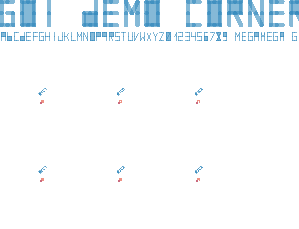
\includegraphics[width=\textwidth]{Content/Masks/EM160509_GOI_Demo_CornerCube.pdf}
            \caption{Advanced Example: Part of the Generated Mask}
            \label{fig:AppendixTXLWizardExampleAdvanced}
        \end{figure}




\end{appendices}




\end{document}